\documentclass{beamer}
\usepackage{beamerthemeshadow}
\usepackage[brazil]{babel}
\usepackage[utf8]{inputenc}
\usepackage{graphicx}
\usepackage[compatibility=false]{caption}
\usepackage{subcaption}

\begin{document}
\title{MC920: Introdução ao Processamento de Imagem Digital}
\author{Martin de Oliveira (118077) \and Rafael Hermano (121286)}
\date{\today}

\frame{\titlepage}

\frame{\frametitle{Números de conexidade}
    \begin{itemize}
        \item Rutovitz
            \[NC = \sum_{k=1}^8 \left| x_k - x_{k+1}\right|\]
        \item Yokoi (4-conexo)
            \[NC = \sum_{k \in V_4} \left| x_k - x_k \cdot x_{k+1} \cdot x_{k+2}\right|\]
        \item Yokoi (4-conexo)
        \[NC = \sum_{k \in V_4} \left| \overline{x_k} - \overline{x_k} \cdot \overline{x_{k+1}} \cdot \overline{x_{k+2}}\right|\]
    \end{itemize}
    \vfill
}
\frame{\frametitle{Números de conexidade}

    \begin{tabular}{cc}
        \begin{minipage}{8cm}
            \begin{figure}[!ht]
                \centering
                \begin{subfigure}[ht]{0.39\textwidth}
                    \fbox{
\includegraphics[width=\textwidth]{img2.png}}
                    \caption{Original}
                \end{subfigure}
                \qquad
                \begin{subfigure}[ht]{0.39\textwidth}
                    \fbox{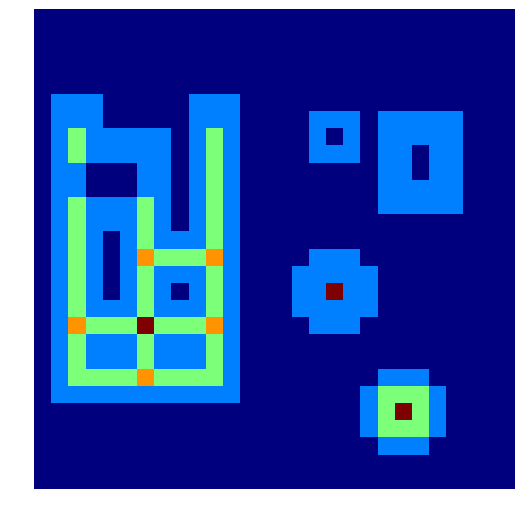
\includegraphics[width=\textwidth]{rutovitz.png}}
                    \caption{Rutovitz}
                \end{subfigure}
                \\
                \begin{subfigure}[ht]{0.39\textwidth}
                    \fbox{
\includegraphics[width=\textwidth]{yokoi4.png}}
                    \caption{Yokoi - 4 conexo}
                \end{subfigure}
                \qquad
                \begin{subfigure}[ht]{0.39\textwidth}
                    \fbox{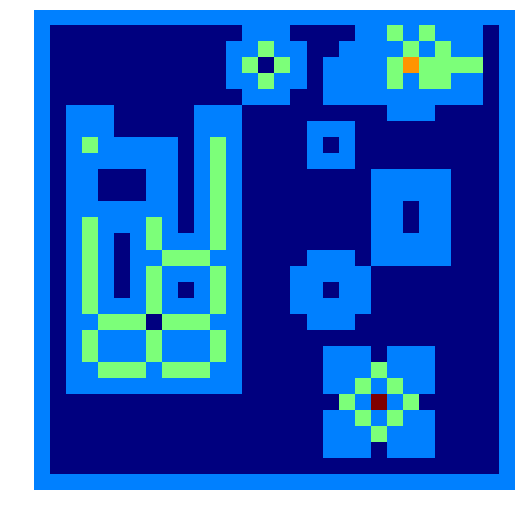
\includegraphics[width=\textwidth]{yokoi8.png}}
                    \caption{Yokoi - 8 conexo}
                \end{subfigure}
            \end{figure}
        \end{minipage}
        & 
        \begin{minipage}{4cm}
            \begin{figure}[!ht]
                \centering
                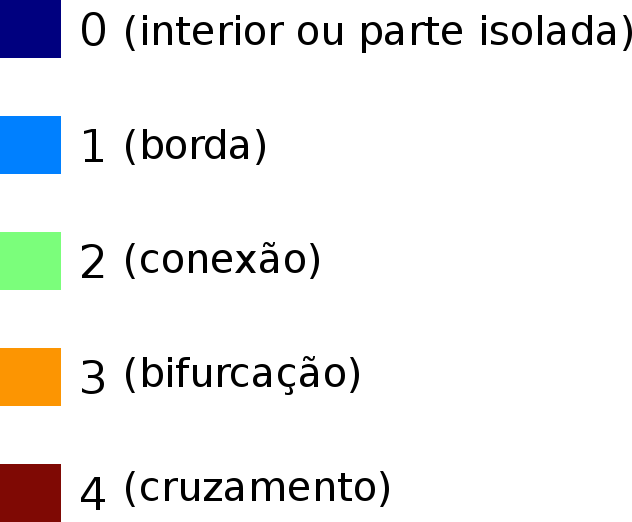
\includegraphics[height=0.5\textheight]{scale.png}
            \end{figure}
        \end{minipage}
    \end{tabular}
}

\frame{\frametitle{Transformada de distância}
    \begin{figure}[!ht]
        \centering
        \begin{subfigure}[ht]{0.45\textwidth}
            
\includegraphics[width=\textwidth]{img.png}
            \caption{Original}
        \end{subfigure}
        \qquad
        \begin{subfigure}[ht]{0.45\textwidth}
            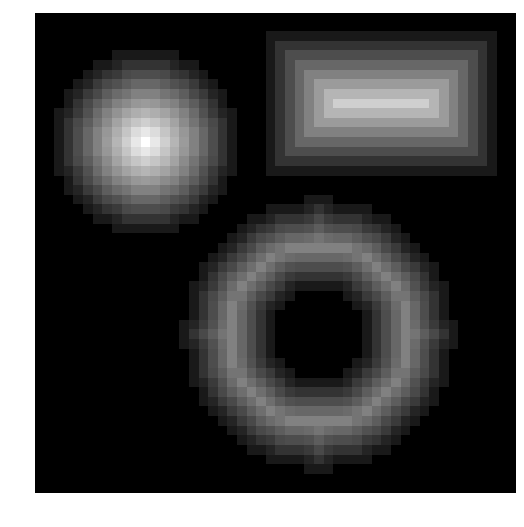
\includegraphics[width=\textwidth]{dist.png}
            \caption{Transformada de distância}
        \end{subfigure}
    \end{figure}
}
\end{document}
